\documentclass{ximera}
%\usepackage{todonotes}

\newcommand{\todo}{}

\usepackage{tkz-euclide}
\tikzset{>=stealth} %% cool arrow head
\tikzset{shorten <>/.style={ shorten >=#1, shorten <=#1 } } %% allows shorter vectors

\usepackage{tkz-tab}  %% sign charts
\usetikzlibrary{decorations.pathreplacing} 

\usetikzlibrary{backgrounds} %% for boxes around graphs
\usetikzlibrary{shapes,positioning}  %% Clouds and stars
\usetikzlibrary{matrix} %% for matrix
\usepgfplotslibrary{polar} %% for polar plots
\usetkzobj{all}
\usepackage[makeroom]{cancel} %% for strike outs
%\usepackage{mathtools} %% for pretty underbrace % Breaks Ximera
\usepackage{multicol}

\usepackage{polynom}



\usepackage[many]{tcolorbox}  %% for titled boxes
\newtcolorbox{xbox}[1]{%
    tikznode boxed title,
    enhanced,
    arc=0mm,
    interior style={white},
    attach boxed title to top center= {yshift=-\tcboxedtitleheight/2},
    fonttitle=\bfseries,
    colbacktitle=white,coltitle=black,
    boxed title style={size=normal,colframe=white,boxrule=0pt},
    title={#1}}


\usepackage{array}
\setlength{\extrarowheight}{+.1cm}   
\newdimen\digitwidth
\settowidth\digitwidth{9}
\def\divrule#1#2{
\noalign{\moveright#1\digitwidth
\vbox{\hrule width#2\digitwidth}}}





\newcommand{\RR}{\mathbb R}
\newcommand{\R}{\mathbb R}
\newcommand{\N}{\mathbb N}
\newcommand{\Z}{\mathbb Z}

%\renewcommand{\d}{\,d\!}
\renewcommand{\d}{\mathop{}\!d}
\newcommand{\dd}[2][]{\frac{\d #1}{\d #2}}
\newcommand{\pp}[2][]{\frac{\partial #1}{\partial #2}}
\renewcommand{\l}{\ell}
\newcommand{\ddx}{\frac{d}{\d x}}
\newcommand{\ddt}{\frac{d}{\d t}}

\newcommand{\zeroOverZero}{\ensuremath{\boldsymbol{\tfrac{0}{0}}}}
\newcommand{\inftyOverInfty}{\ensuremath{\boldsymbol{\tfrac{\infty}{\infty}}}}
\newcommand{\zeroOverInfty}{\ensuremath{\boldsymbol{\tfrac{0}{\infty}}}}
\newcommand{\zeroTimesInfty}{\ensuremath{\small\boldsymbol{0\cdot \infty}}}
\newcommand{\inftyMinusInfty}{\ensuremath{\small\boldsymbol{\infty - \infty}}}
\newcommand{\oneToInfty}{\ensuremath{\boldsymbol{1^\infty}}}
\newcommand{\zeroToZero}{\ensuremath{\boldsymbol{0^0}}}
\newcommand{\inftyToZero}{\ensuremath{\boldsymbol{\infty^0}}}



\newcommand{\numOverZero}{\ensuremath{\boldsymbol{\tfrac{\#}{0}}}}
\newcommand{\dfn}{\textbf}
%\newcommand{\unit}{\,\mathrm}
\newcommand{\unit}{\mathop{}\!\mathrm}
\newcommand{\eval}[1]{\bigg[ #1 \bigg]}
\newcommand{\seq}[1]{\left( #1 \right)}
\renewcommand{\epsilon}{\varepsilon}
\renewcommand{\iff}{\Leftrightarrow}

\DeclareMathOperator{\arccot}{arccot}
\DeclareMathOperator{\arcsec}{arcsec}
\DeclareMathOperator{\arccsc}{arccsc}
\DeclareMathOperator{\si}{Si}
\DeclareMathOperator{\proj}{proj}
\DeclareMathOperator{\scal}{scal}


\newcommand{\tightoverset}[2]{% for arrow vec
  \mathop{#2}\limits^{\vbox to -.5ex{\kern-0.75ex\hbox{$#1$}\vss}}}
\newcommand{\arrowvec}[1]{\tightoverset{\scriptstyle\rightharpoonup}{#1}}
\renewcommand{\vec}{\mathbf}
\newcommand{\veci}{\vec{i}}
\newcommand{\vecj}{\vec{j}}
\newcommand{\veck}{\vec{k}}
\newcommand{\vecl}{\boldsymbol{\l}}

\newcommand{\dotp}{\bullet}
\newcommand{\cross}{\boldsymbol\times}
\newcommand{\grad}{\boldsymbol\nabla}
\newcommand{\divergence}{\grad\dotp}
\newcommand{\curl}{\grad\cross}
%\DeclareMathOperator{\divergence}{divergence}
%\DeclareMathOperator{\curl}[1]{\grad\cross #1}


\colorlet{textColor}{black} 
\colorlet{background}{white}
\colorlet{penColor}{blue!50!black} % Color of a curve in a plot
\colorlet{penColor2}{red!50!black}% Color of a curve in a plot
\colorlet{penColor3}{red!50!blue} % Color of a curve in a plot
\colorlet{penColor4}{green!50!black} % Color of a curve in a plot
\colorlet{penColor5}{orange!80!black} % Color of a curve in a plot
\colorlet{fill1}{penColor!20} % Color of fill in a plot
\colorlet{fill2}{penColor2!20} % Color of fill in a plot
\colorlet{fillp}{fill1} % Color of positive area
\colorlet{filln}{penColor2!20} % Color of negative area
\colorlet{fill3}{penColor3!20} % Fill
\colorlet{fill4}{penColor4!20} % Fill
\colorlet{fill5}{penColor5!20} % Fill
\colorlet{gridColor}{gray!50} % Color of grid in a plot

\newcommand{\surfaceColor}{violet}
\newcommand{\surfaceColorTwo}{redyellow}
\newcommand{\sliceColor}{greenyellow}




\pgfmathdeclarefunction{gauss}{2}{% gives gaussian
  \pgfmathparse{1/(#2*sqrt(2*pi))*exp(-((x-#1)^2)/(2*#2^2))}%
}


%%%%%%%%%%%%%
%% Vectors
%%%%%%%%%%%%%

%% Simple horiz vectors
\renewcommand{\vector}[1]{\left\langle #1\right\rangle}


%% %% Complex Horiz Vectors with angle brackets
%% \makeatletter
%% \renewcommand{\vector}[2][ , ]{\left\langle%
%%   \def\nextitem{\def\nextitem{#1}}%
%%   \@for \el:=#2\do{\nextitem\el}\right\rangle%
%% }
%% \makeatother

%% %% Vertical Vectors
%% \def\vector#1{\begin{bmatrix}\vecListA#1,,\end{bmatrix}}
%% \def\vecListA#1,{\if,#1,\else #1\cr \expandafter \vecListA \fi}

%%%%%%%%%%%%%
%% End of vectors
%%%%%%%%%%%%%

%\newcommand{\fullwidth}{}
%\newcommand{\normalwidth}{}



%% makes a snazzy t-chart for evaluating functions
%\newenvironment{tchart}{\rowcolors{2}{}{background!90!textColor}\array}{\endarray}

%%This is to help with formatting on future title pages.
\newenvironment{sectionOutcomes}{}{} 



%% Flowchart stuff
%\tikzstyle{startstop} = [rectangle, rounded corners, minimum width=3cm, minimum height=1cm,text centered, draw=black]
%\tikzstyle{question} = [rectangle, minimum width=3cm, minimum height=1cm, text centered, draw=black]
%\tikzstyle{decision} = [trapezium, trapezium left angle=70, trapezium right angle=110, minimum width=3cm, minimum height=1cm, text centered, draw=black]
%\tikzstyle{question} = [rectangle, rounded corners, minimum width=3cm, minimum height=1cm,text centered, draw=black]
%\tikzstyle{process} = [rectangle, minimum width=3cm, minimum height=1cm, text centered, draw=black]
%\tikzstyle{decision} = [trapezium, trapezium left angle=70, trapezium right angle=110, minimum width=3cm, minimum height=1cm, text centered, draw=black]

\author{Bart Snapp\and Nela Lakos}
\license{Creative Commons 3.0 By-NC}
\acknowledgement{https://www.whitman.edu/mathematics/calculus/}
  \outcome{Interpret an optimization problem as the procedure used to make a system or design as effective or functional as possible.}
  \outcome{Set up an optimization problem by identifying the objective function and appropriate constraints.}
  \outcome{Solve optimization problems by finding the appropriate absolute extremum.}
  \outcome{Solve basic word problems involving maxima or minima.}
\begin{document}
\begin{exercise}

  A rectangle is inscribed in the ellipse
  \[
  \frac{x^2}{3}+\frac{y^2}{5}=1
  \]
  so that two of its edges are parallel to the $x$-axis, and the other two are parallel to the $y$-axis.
  Find the dimensions of the rectangle with the largest area.
  \begin{hint}
  \begin{image}
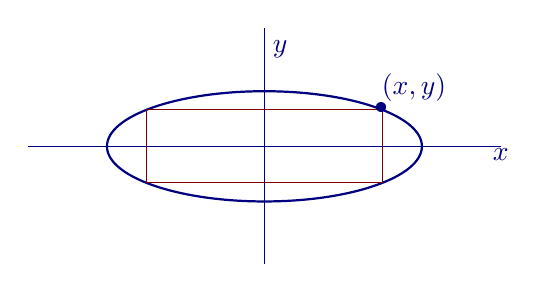
\begin{tikzpicture}
\coordinate (c) at (1.495,2.492);
\draw[penColor, thick] (0,2) ellipse (2 and .7);
%\draw[very thick,penColor!20!background] (2,-2) arc (0:180:2 and .7);% top half of ellipse
%\draw[very thick,penColor] (-2,-2) arc (180:360:2 and .7);% bottom half of ellips
\draw[penColor,  thin] (-3,2) -- (3,2);
\draw[penColor,  thin] (0,0.5) -- (0,3.5);
\draw[penColor2,  thin] (-3/2,1.57+2/2.24) -- (3/2,1.57+2/2.24);
\draw[penColor2,  thin] (-3/2,2.43-2/2.24) -- (3/2,2.43-2/2.24);
\draw[penColor2,  thin]  (-3/2,2.43-2/2.24) -- (-3/2,1.57+2/2.24);
\draw[penColor2,  thin]  (3/2,2.43-2/2.24) -- (3/2,1.57+2/2.24);
    \draw [color=penColor,fill=penColor] (1.5,3);  %% closed hole   
    \node [above,penColor] at (0.2,3) {$y$};
 \node [above,penColor] at (3,1.7) {$x$};
  \node [above,penColor] at (1.9,2.45) {$(x,y)$};
\node at (c) [penColor] {\small\textbullet};
\end{tikzpicture}
\end{image}
\end{hint}
\begin{hint}
Area of the rectangle
 $A=2x\cdot 2y$. 
 We will express $A$ as a function of, say, $x$.
Note that $x$ and $y$ satisfy the equation of the ellipse, so
 \[
y^2=5-  \frac{5x^2}{3}
  \]
Since in our figure $y\ge0$, we have 
 \[
y=\sqrt{5-  \frac{5x^2}{3}}
  \]
\end{hint}
\begin{hint}
Now
$A(x)=2x\cdot 2\sqrt{5-  \frac{5x^2}{3}}$.

The domain of $A=\left[0,\answer{\sqrt{3}}\right]$.
\end{hint}
\begin{hint}
We have to find the critical points of $A$.


$A'(x)=4\cdot \sqrt{5-  \frac{5x^2}{3}}+\frac{4x}{2\sqrt{5-  \frac{5x^2}{3}}}\cdot \left(-\frac{10}{3}x\right)$.
If we simplify $A'(x)$, we get

$A'(x)=4\cdot \sqrt{5-  \frac{5x^2}{3}}-\frac{20x^2}{3\sqrt{5-  \frac{5x^2}{3}}}$, 

and if we simplify again, we get

$A'(x)=\frac{60-40x^2}{3\sqrt{5-  \frac{5x^2}{3}}}$

The function $A$ has the only critical point at $x=\sqrt{\frac{\answer{3}}{2}}$.
\end{hint}
\begin{hint}

Since the domain of $A$ is a closed interval $\left[0,\answer{\sqrt{3}}\right]$, 
we have to evaluate the function $A$ at the end points and at the critical point:
 \[
A(0)=0
  \]
  \[
A(\sqrt{3})=0
  \]
  \[
A\left(\sqrt{\frac{\answer{3}}{2}}\right)=4\sqrt{\frac{\answer{3}}{2}}\sqrt{5-  \frac{5}{2}}=2\sqrt{15}.
  \]
  So, the maximum is attained at the critical point.
\end{hint}
  \begin{prompt}
  \begin{align*}
  \text{base}&= \answer{\sqrt{6}}\\
  \text{height} &= \answer{\sqrt{10}}
  \end{align*}
  \end{prompt}
\end{exercise}
\end{document}
